\chapter{Simulating with Fussy.jl}

\label{chapter:fussy}

Fussy.jl is a 0-D \underline{fus}ion \underline{sy}stems code written using the Julia language. The reason for choosing Julia over say Matlab and Python was due to metaprogramming concerns and its tight-knit  computational community, respectively. Incorporating the model used throughout this paper, the code is quick to run and matches more sophisticated frameworks with high fidelity.

This chapter will be broken down into three steps. The first is getting a user up and running with the code. Once the user gets to this point, hopefully they will wonder how the code is structured. This will be the second step. The final step will be explaining the various functions callable on reactor objects -- the atomic data structure for Fussy.jl.

\section{Getting the Code to Work}

The hardest step of any codebase is getting it up and running. These instructions should get a user to a point where they are a few internet searches away from a working copy of Fussy.jl. As an aide, you can view an interactive collection of Fussy.jl Jupyter notebooks at the following website:

{\centering \href{http://fusion.codes}{www.fusion.codes} \par }

Although \href{http://fusion.codes}{fusion.codes} is a nice tool for viewing this document's results, it is a little slow for producing new data -- and it also lacks a method for storing it. Therefore, an advanced user should first download a copy of Julia from:

{\centering \href{https://julialang.org/downloads}{julialang.org/downloads} \par }

Currently the Fussy.jl codebase is written using \texttt{v0.6}, but should be \texttt{v1.0} compatible by 2019. Using Julia nomenclature, Fussy.jl is a Julia package. It can be cloned using Julia conventions from the following Github repository:

{\centering \href{https://github.com/djsegal/Fussy.jl.git}{https://github.com/djsegal/Fussy.jl.git} \par }

Once the Fussy.jl package has been cloned into your Julia package library, you should be able to access it through the Julia REPL or a Jupyter notebook. You can now reproduce every plot in this text. A quick test to see if your code works is:
\begin{addmargin}[1.5em]{1.5em}
\texttt{using Fussy \\
cur\_reactor = Reactor(15) \\
@assert cur\_reactor.T\_bar == 15 \\
println("It works!")
}
\end{addmargin}

If the code works, you should get a "It works!" message as output.

\section{Sorting out the Codebase}

Assuming the user got to this section, the code works and now you want to know what you can do with it. The place to start is in the \texttt{src} folder, again viewable online at:

{\centering \href{http://git.io/tokamak}{git.io/tokamak} \par }

Within the \texttt{src} folder are several subfolders as well as a few files (e.g.\ Fussy.jl and defaults.jl). In an attempt to not bore the reader, we will be painting with thick brushstrokes. Further, the \texttt{methods} subfolder will be the topic of the next section -- as most involve calls on a reactor object.

\subsection{Typing out Structures}

The place to start in any modeling framework is its data structures. These type definitions allow the building of nested hierarchies of constructed objects. The most atomic of these is the Reactor struct, but several other ones allow for solving broader scoped questions (i.e.\ Scans, Sensitivities, and Samplings.)

\subsubsection{The Reactor Structure}

Reactors are the most atomic data structure in this fusion systems model. They store all the fields needed to represent a reactor as it exists in reactor space. This obviously includes its temperature, current, and radius, but also includes derived quantities, such as the cost-per-watt and bootstrap fraction. They can be initialized, solved, updated, and honed. Most other data structures are just wrappers to hold these reactors -- they are described next.

\subsubsection{The Scan Structure}

A Scan object is a collection of reactors made from scanning a list of temperatures. For example, a scan of five temperatures from 5 keV to 25 keV would result in several arrays of five reactors. Most often, one of these lists would correspond to beta reactors, one to kink reactors, and one to wall loading reactors. There may then be fewer than five reactors in a list if some of the reactors are invalid or fundamentally unsolvable.

This is the data structure that produces the various comparison plots in the results.

\subsubsection{The Sensitivity Structure}

Sensitivity studies are how computationalists test the effect of changing a variable over multiple values -- i.e.\ do a 20\% sensitivity around the H factor. Like Scans, Sensitivities store various lists of reactors, each corresponding to an interesting data point. These include limit reactors where the beta limit and kink limit are just satisfied or when the beta limit and wall loading are just satisfied. Additionally, they include the minimum capital cost reactors and the minimum cost-per-watt ones.

\subsubsection{The Sampling Structure}

The Sampling struct was created to do simple Monte Carlo runs over a reactor's \replaced{static}{fixed} values. While sensitivities only allow one variable to change at a time, samplings randomly assign a list of variables to some neighborhood of possible values. These are how the scatter plots are made. Succinctly, where sensitivity studies show local changes to variables, Monte Carlo samplings show global trends in reactor design.

\subsubsection{The Equation Structure}

In order to store the various equations from \cref{table:eq} is the Equation Struct. It stores the $\gamma$ exponents for: $R_0$, $B_0$, and $I_P$. -- as well as the function representing G($\overline T$). Repeated these are the unknowns in:
\begin{equation}
	\tag{\ref{eq:rbi}}
	R_0^{\, \gamma_R} \cdot B_0^{\, \gamma_B} \cdot I_P^{\, \gamma_I} = G( \overline T )
\end{equation}
Concretely, there are 16 objects that use this struct -- one for each equation (e.g.\ for fusion power, the beta limit, and temperature assignment).

\subsubsection{The Equation Set Structure}

The step up from the Equation struct are the Equation Sets. These collections of three equations allow $R_0$, $B_0$, and maybe $I_P$ to be substituted out of the current balance root-solving equation. This is where \cref{eq:case_1_R,eq:case_1_B,eq:case_1_I,eq:case_1_gamma,eq:case_2_R,eq:case_2_B,eq:case_2_gamma} come into play.

\subsection{Referencing Input Decks and Solutions}

With more than twenty \replaced{static}{fixed} variables in the model, the range of tokamak reactors is basically infinite. To help users build a net of designs to explore reactor space are seven input decks. These are the ones given in the results: ARC, ACT I /II, DEMO Steady/Pulsed, Proteus and Charybdis. Coupled with the non-prototype reactors are solution reactors that store various quantities from the original papers (e.g.\ $P_F$, $f_{BS}$, $R_0$). These are how the comparison tables were constructed.

\subsection{Acknowledging Utility Functions}

For the uninitiated, utility functions are grab bag functions that do not really belong in a codebase -- but do anyway. This sentiment does not mean they are worthless, just not fusion related at all. In Fussy.jl, the most notable are a normalized integral calculator, a filter that includes numeric tolerances, and a robust root solver.

Although since incorporated into the official Roots.jl package, \texttt{find\_roots} allows finding an arbitrary number of roots within a bounded range. This was needed because many roots can be found at various levels of the reactor solving problem -- i.e.\ for $I_P$, $\overline T$, $\eta_{CD}$, etc.

\subsection{Mentioning Base Level Files}

In addition to subdirectories within the \texttt{src} folder are three files: Fussy.jl, abstracts.jl, and defaults.jl. Fussy.jl is the package's main file that actually stores the Fussy module. While, abstracts.jl stores various abstract structures that help clean up other files.

Finally, defaults.jl stores various default values that are important to the codebase. For example, this is where the various scaling law exponents are stored. It is also where the bounding values for the different root solving problems live. These include minimum and maximum values for: $I_P$, $\overline T$, $\eta_{CD}$.

Now that a majority of the files have been discussed, we can turn to the reactor methods. These constitute most of the interesting functionality within the codebase.

\section{Delving into Reactor Methods}

The reactor is the most atomic data structure in this model. It therefore makes sense that it has many instance methods. These include all the coefficients, fluxes, powers, etc. It also includes methods that solve a reactor, perform a match on some field's value, or converge $\eta_{CD}$ to self-consistency. The various subdirectories within the \texttt{src/methods/reactors} folder will now be discussed.

\subsubsection{Calculations}

The calculation subdirectory of reactor methods are used to set various important values in the solver. For \replaced{dynamic}{floating} variables, these include: $\overline n$, $R_0$, $B_0$, and $I_P$. This folder also includes the calculation of the Bosch-Hale reactivity and the Ehst-Karney current drive efficiency.

\subsubsection{Coefficients and Composites}

The coefficients and composites directories correspond to the model's \replaced{static}{fixed} and \replaced{dynamic}{floating} coefficients, respectively. For clarity, \replaced{static}{fixed} coefficients, including $K_n$ and $K_{CD}$, were labeled with a K. Whereas, \replaced{dynamic}{floating} coefficients then started with G's -- i.e.\ $G_{PB}$ and $G_V$.

\subsubsection{Fluxes and Powers}

Within flux balance and power balance were around a dozen terms or sub-terms. Although not directly used in the conservation equations, sub-terms are used to compare the model to ones from the literature. For clarity, fluxes include: $\Phi_{CS}$, $\Phi_{PF}$, $\Phi_{RU}$, $\Phi_{FT}$, $\Phi_{res}$, and $\Phi_{ind}$. The powers, then, include: $P_F$, $P_{BR}$, $P_\kappa$, $P_{src}$, $P_W$, etc.

\subsubsection{Profiles}

The next collection of reactor methods are the various profiles. Most obviously, these include radial plasma profiles for density, temperature, and current. However, this folder also includes the magnetic field strength as a function of radius -- as was used within current drive efficiency calculations.

\subsubsection{Geometries}

Additionally, there are many geometric relations. These include the various tokamak thicknesses: a, b, c, d -- as well as the radius and height of the central solenoid. This group also includes the volume, perimeter, surface area, and cross-sectional area. It also includes the many subscripted fields. For example, the elongation (i.e.\ $\kappa_{95}$) includes the following alternative definitions: $\kappa_X$, $\kappa_P$, and $\kappa_\tau$

\subsubsection{Formulas}

The final set of reactor methods are formulas that do not really fit anywhere else. If a method is not related to geometry, power, calculations, etc, it ends up here. For example, this group includes: $\beta_N$, $f_{BS}$, $C_W$, and $\tau_E$. Total, there are around 25 formulas -- as of the writing of this document.

\section{Demonstrating Code Usage}

Now that the Fussy.jl package has been described in detail, the final step is showing a simple example that can recreate a figure from the results chapter. This will closely match the Jupyter notebook available at:

{\centering \href{https://git.io/fussy_sensitivity}{www.git.io/fussy\_sensitivity} \par }

Our goal will be to make a cost curve for the ARC reactor as a function of H -- a so called sensitivity study plot.

\subsection{Initializing the Workspace}

The first step for any Fussy.jl Jupyter notebook is loading the required packages -- i.e.\ the Fussy.jl and Plots.jl packages. This can be done using the following commands:\footnote{The \texttt{addprocs} and \texttt{@everywhere} commands are to parallelize the code. This is because \texttt{addprocs(6)} activates 6 worker processes and \texttt{@everywhere Fussy.jl} adds Fussy.jl to the main kernel and worker processes.}

\begin{addmargin}[1.5em]{1.5em}
\texttt{addprocs(6) \\
@everywhere using Fussy \\
using Plots
}
\end{addmargin}

The Plots.jl package may take a minute to load -- similar to Matlab's initial boot time. If the kernel raises an error about Plots.jl not being installed, use the following lines:

\begin{addmargin}[1.5em]{1.5em}
\texttt{import Pkg \\
Pkg.add("Plots")
}
\end{addmargin}

\subsection{Running a Study}

Now that the necessary packages have been loaded, we can move on to actually running the sensitivity study. We will split this command into two steps to make it more explicit.

The first step will be making several variables that store: boolean flags, numbers, and symbols -- which are like strings, but prefaced with a colon (\texttt{:}) instead of surrounded by double quotes (\texttt{"}).

\begin{addmargin}[1.5em]{1.5em}
\texttt{cur\_param = :H \\
cur\_deck = :arc \\
is\_pulsed = false \\
is\_consistent = true \\
cur\_sensitivity = 1.0 \\
cur\_num\_points = 41
}
\end{addmargin}

These six variables almost completely describe a sensitivity study. The first two saw we are using the ARC reactor deck and running a sensitivity over the H-factor parameter. Next, the two boolean values refer to the reactor (1) being treated as pulsed or steady-state and (2) wether to handle $\eta_{CD}$ self-consistently.\footnote{Note that, currently, a pulsed reactor cannot be self-consistent in $\eta_{CD}$ -- it therefore causes an error.} Ergo, what these two flags do is make sure ARC is being handled as a steady-state reactor with a self-consistent $\eta_{CD}$. The last two variables are then ways to change the sensitivity of the study (with $1.0 \rightarrow 100\%$) and the number of reactors it will produce (i.e.\ 41).

Now all six of these variables can be piped into a call to the \texttt{Study} struct to start running the sensitivity study:

\begin{addmargin}[1.5em]{1.5em}
\texttt{cur\_study = Study( \\
\-\ \-\ cur\_param, \\
\-\ \-\ deck = cur\_deck, \\
\-\ \-\ is\_pulsed = is\_pulsed, \\
\-\ \-\ is\_consistent = is\_consistent, \\
\-\ \-\ sensitivity = cur\_sensitivity, \\
\-\ \-\ num\_points = cur\_num\_points \\
)
}
\end{addmargin}

Note here that the equal signs inside the parentheses are called keyword arguments, which are common to most modern programming languages. After executing the command, the code will need to run for a few minutes.

\subsection{Extracting Results}

At this point, a user should have a completed sensitivity study they wish to plot. To make the plot useful, the study data structure first has to be unpacked and its contents cleaned. This is the goal of this subsection.

First and foremost, a study has four families of reactors within it: beta-wall (i.e.\ "wall"), beta-kink (i.e.\ "kink"), minimum capital cost (i.e.\ "W\_M"), and minimum cost-per-watt (i.e.\ "cost"). Therefore, we will extract these reactor lists into a new dictionary data structure:

\begin{addmargin}[1.5em]{1.5em}
\texttt{cur\_dict = Dict() \\ ~ \\
cur\_dict["Beta-Wall"] = cur\_study.wall\_reactors \\
cur\_dict["Beta-Kink"] = cur\_study.kink\_reactors \\ ~ \\
cur\_dict["Min Cost-per-Watt"] = cur\_study.cost\_reactors \\
cur\_dict["Min Capital Cost"] = cur\_study.W\_M\_reactors
}
\end{addmargin}

Next, we will want to filter out all the invalid reactors that constitute non-physically realizable ones. These would likely be reactors that could fit in your hand or take up a whole city block.

\begin{addmargin}[1.5em]{1.5em}
\texttt{for (cur\_key, cur\_value) in cur\_dict \\
\-\ \-\ cur\_dict[cur\_key] = filter( \\
\-\ \-\ \-\ \-\ cur\_reactor -> cur\_reactor.is\_valid, \\
\-\ \-\ \-\ \-\ deepcopy(cur\_value) \\
\-\ \-\ ) \\
end
}
\end{addmargin}

\subsection{Plotting Curves}

Our goal is now to turn our unpacked, clean reactor lists into plots -- i.e.\ measuring costs-per-watt as a function of H. For simplicity, this will lack a lot of the features shown in the Jupyter notebook from the beginning of the section. Additionally, we will be doing it in an iterative process made possible by the Plots.jl framework.

The first step is simply making a plot object

\begin{addmargin}[1.5em]{1.5em}
\texttt{cur\_plot = plot()}
\end{addmargin}

After execution, this should produce the plank 2-D plot shown in \cref{fig:example_1}.

\begin{figure}
	\centering
	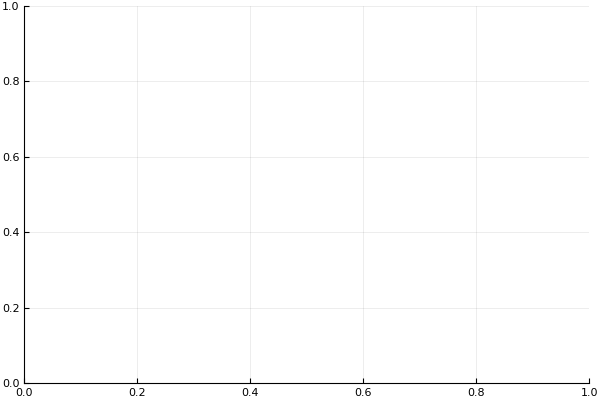
\includegraphics[width=0.7\textwidth]{images/example_1}
	\caption{A Blank Plot} ~\\
	\small A simple 2-D plot with no labels or data.
	\label{fig:example_1}
\end{figure}

Next we will add a simple title and labels for the axes:

\begin{addmargin}[1.5em]{1.5em}
\texttt{title!("ARC") \\ ~ \\
xlabel!("H") \\
ylabel!("Cost")
}
\end{addmargin}

The exclamation marks ensure this title and the labels are added to the \texttt{cur\_plot}. Upon execution, you should see a plot with this information (\cref{fig:example_2}).

\begin{figure}
	\centering
	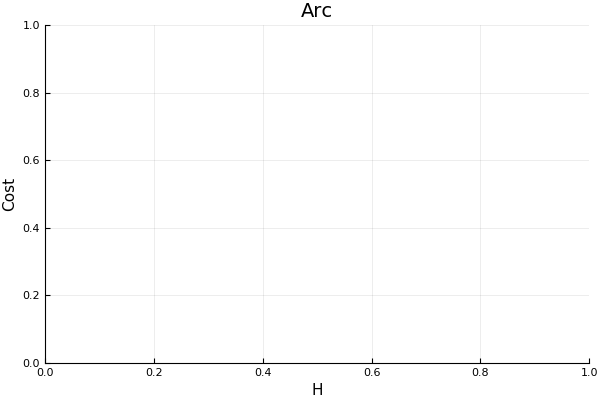
\includegraphics[width=0.7\textwidth]{images/example_2}
	\caption{An Empty Plot} ~\\
	\small A simple 2-D plot with labels, but no data.
	\label{fig:example_2}
\end{figure}

Now we will loop over the dictionary of reactors and add them one at a time.

\begin{addmargin}[1.5em]{1.5em}
\texttt{for (cur\_key, cur\_value) in cur\_dict \\
\-\ \-\ cur\_x = map(cur\_reactor -> cur\_reactor.H, cur\_value) \\
\-\ \-\ cur\_y = map(cur\_reactor -> cur\_reactor.cost, cur\_value) \\
\-\ \-\ plot!(cur\_x, cur\_y, label=cur\_key) \\
end \\
plot!()
}
\end{addmargin}

This results in the not very useful plot shown in \cref{fig:example_3}. Note that each label is exactly the key assigned to it in \texttt{cur\_dict}.

\begin{figure}
	\centering
	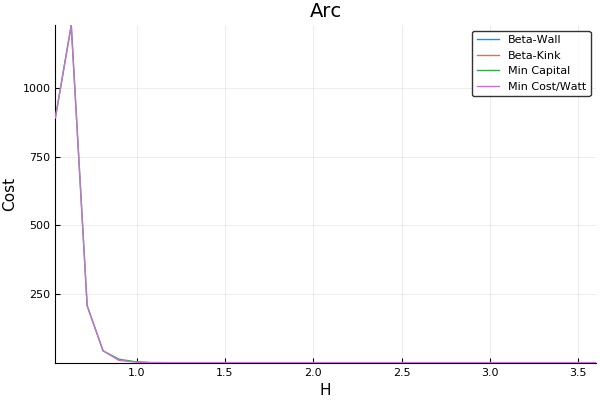
\includegraphics[width=0.7\textwidth]{images/example_3}
	\caption{An Unscaled Plot} ~\\
	\small A simple 2-D plot with Bad Limits.
	\label{fig:example_3}
\end{figure}

The final step is adding proper limits to make what is going on obvious to the reader:

\begin{addmargin}[1.5em]{1.5em}
\texttt{ylims!(0, 0.03)}
\end{addmargin}

\begin{figure}
	\centering
	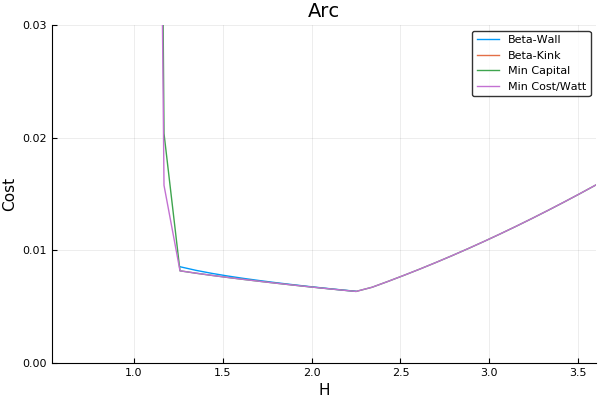
\includegraphics[width=0.7\textwidth]{images/example_4}
	\caption{A Scaled Plot} ~\\
	\small An example plot showing cost as a function of the H factor.
	\label{fig:example_4}
\end{figure}

The addition of which can be seen in \cref{fig:example_4}.

This completes the example. At this point, you should now be able to use every feature of Fussy.jl. Good luck!
